% !TeX spellcheck = sv_SE
% !TeX document-id = {a836f75a-a0c6-4045-88b1-6cb4916dad52}
% !TeX TXS-program:compile = txs:///pdflatex/[--shell-escape]
% !TeX TXS-program:bibliography = txs:///biber

\documentclass[]{scrreprt}

\usepackage[backend=biber]{biblatex}
\usepackage[swedish,english]{babel}
\usepackage[utf8]{inputenc}
\usepackage{minted}
\usepackage{graphicx}
\usepackage[iso]{datetime}
\usepackage{amsmath}
\usepackage{mathtools}

%\usepackage[hidelinks]{hyperref}
\usepackage{bookmark}
\usepackage{lastpage}
\usepackage{subcaption}
\usepackage{accsupp}
\usepackage{attachfile}
\usepackage{rotating}
\usepackage{pdflscape}
\usepackage{siunitx}
\usepackage[toc,page]{appendix}
\usepackage{etoc}


\usepackage{etoolbox}
\makeatletter
\patchcmd{\scr@startchapter}{\if@openright\cleardoublepage\else\clearpage\fi}{}{}{}
\makeatother
% roman numeral
\newcommand{\RON}[1]{%
	\textup{\uppercase\expandafter{\romannumeral#1}}%
}

% Title Page
\title{Roadster - R2}
\author{Gardström Emil \and Wallin Dennis}
\subtitle{Beräkningsvetenskap \RON{1}}
\titlehead{\Large Uppsala Universitet\hfill KandMa, Grupp 4}

\addbibresource{roadster.bib}
\begin{document}
\etocdepthtag.toc{mtchapter}
\etocsettagdepth{mtchapter}{subsection}
\etocsettagdepth{mtappendix}{none}
\maketitle
\selectlanguage{english}
%\begin{abstract}
%
%\end{abstract}
\selectlanguage{swedish}
\tableofcontents
\chapter{Inledning}
Detta projekt är en undersökning på räckvidden en elbil har givet data från en specifik väg och bilens laddning. Bilen som används är en \textit{Tesla Roadster} som har ett batteri på \SI{55}{\kilo\watt\hour}
\chapter{Resultat}
\section{Approximation}
För att få fram elförbrukningen och vid en viss hastighet använder vi data från elbilen som innehåller konsumptionen i enheten \si{\watt\hour\per\kilo\meter}.
För att interpolera denna data används \mintinline{matlab}{spline} funktionen. Passningen kan ses i figur~\ref{fig:rgraph}.
Analysering av denna data ger oss den hastighet som tillåter längsta färden med ett fulladdat batteri, \SI{659.48}{\kilo\meter} under \SI{28.7}{\kilo\meter\per\hour}.
% Fix, this looks really bad
\begin{figure}[H]
	\caption{Utskrift 1 från \textit{part1.m}}
	\label{fig:rgraph}
	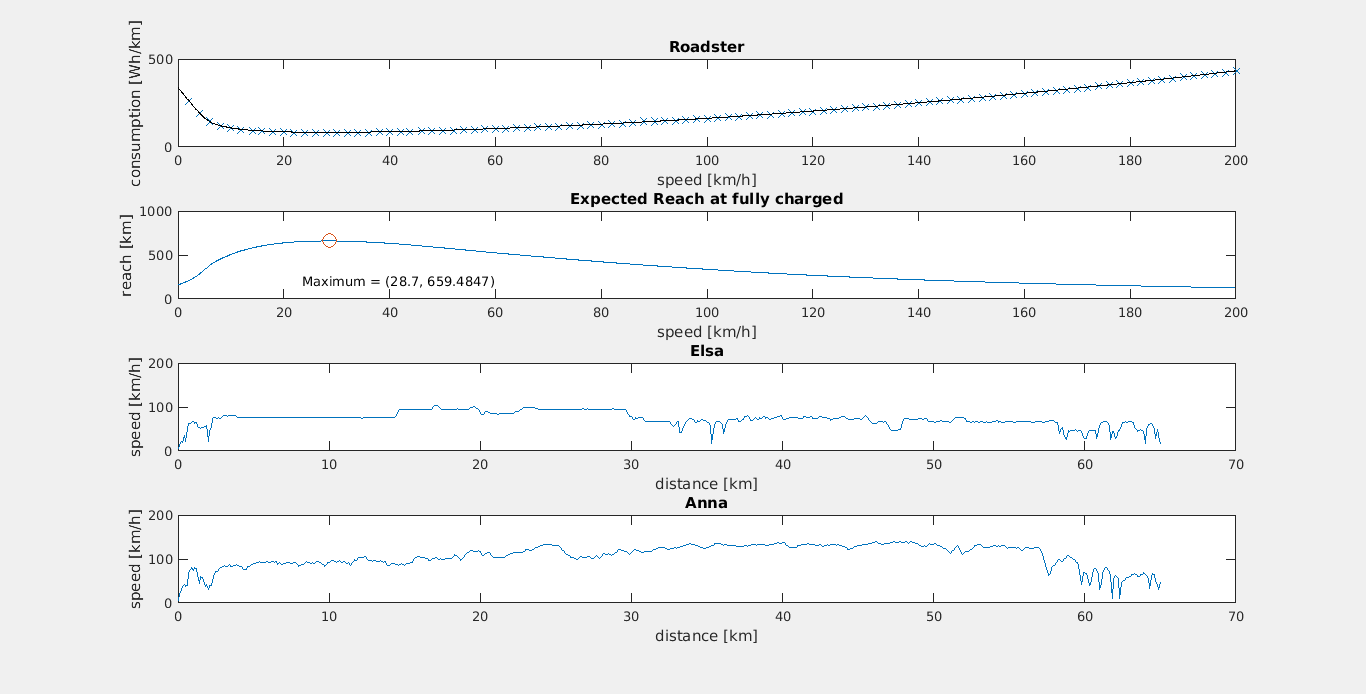
\includegraphics[width=1.2\textwidth]{roadster/part1.png}
\end{figure}
Vi har även fått in data från färden på en väg av två källor. Anna har åkt \SI{65.2162}{\kilo\meter} och Elsa har åkt \SI{65.0040}{\kilo\meter}. Denna data innehåller hastigheten som bilen färdades i efter en viss sträcka. Se figur~\ref{fig:ea_graph}. Även dessa data interpoleras.
\begin{figure}[H]
	\caption{Utskrift 2 från \textit{part1.m}}
	\label{fig:ea_graph}
	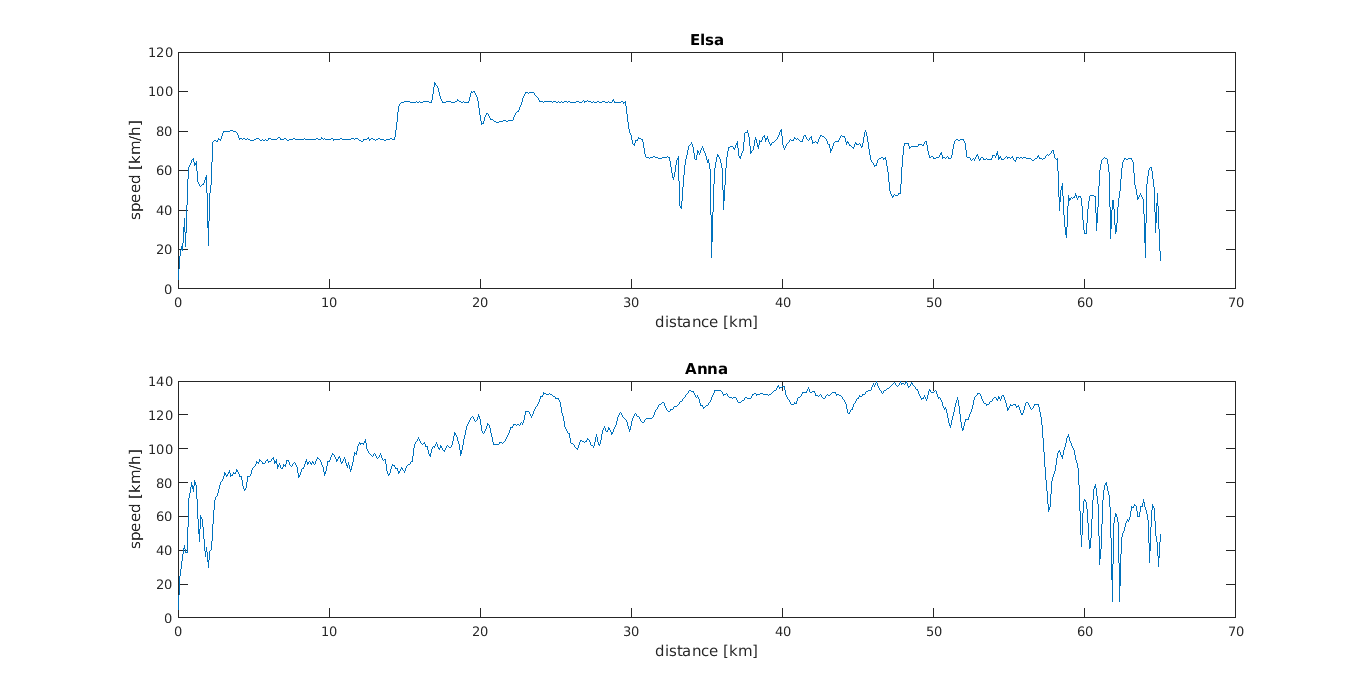
\includegraphics[width=1.2\textwidth]{roadster/elsa_anna.png}
\end{figure}
\section{Integration}
För att uppskatta tiden det tar att anlända och konsumptionen som bilen använder under en resa använder vi oss av en integrerings teknik kallad ~Simpsons adaptiva lag.\cite[]{asimpson}
För tiden får vi integralen
\[ T(x) = \int_0^x \dfrac{1}{v(s)} \, ds \]
och för den totala konsumptionen har vi integralen
\[ E(x) = \int_0^x c(v(s)) \, ds \]
där \(v(s)\) är hastigheten \si{\kilo\meter\per\hour} efter en sträcka \(s\) \si{\kilo\meter} och \(c(v)\) är konsumptionen \si{\watt\hour} vid en hastighet \si{\kilo\meter\per\hour}.\\
Vi ser i figur~\ref{fig:conv} att vår approximering av integrationen är i större del lik \(h^2\), vilket är förväntat av Simpsons. Vi använder oss av $256$ intervall för att integrera då det värdet är det lägsta antalet intervall som är inom en acceptabel tolerans av 2 värdesiffror. Detta var jämfört manuellt med matlabs egna \mintinline{matlab}{integral} som är mer precis. Det tar \SI{0.6990}{\hour} för Anna att åka sin sträcka och \SI{0.9993}{\hour} för Elsa. De förbrukar \SI{11.9443}{\kilo\watt\hour} respektive \SI{8.0403}{\kilo\watt\hour}.
\begin{figure}
	\caption{Utskrift  från \textit{part2.m}}
	\label{fig:conv}
	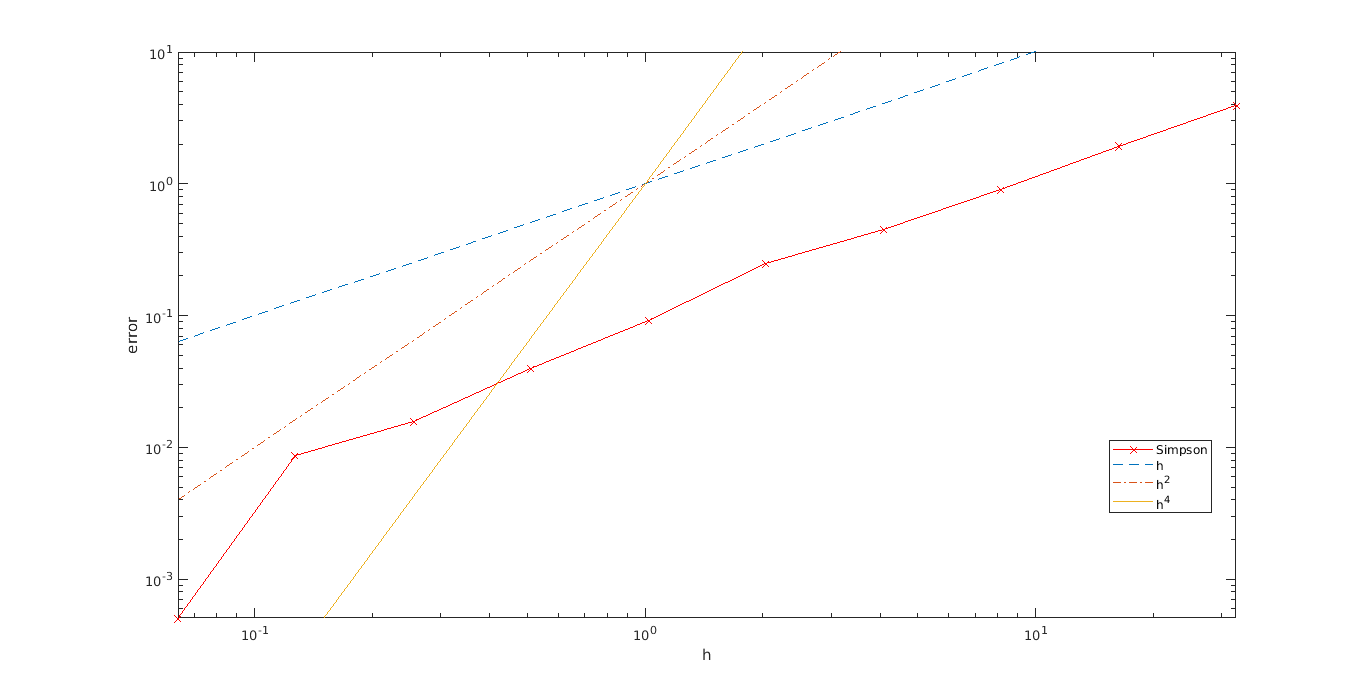
\includegraphics[width=1.2\textwidth]{roadster/conv.png}
\end{figure}
\section{Rotlösning}
För att ta reda på hur långt bilen kommer på \SI[number-math-rm = \mathnormal,parse-numbers=false]{t}{\hour}
eller hur långt bilen kommer med en laddning på \SI[number-math-rm = \mathnormal,parse-numbers=false]{c}{\kilo\watt\hour}
kan vi använda oss av rötterna till den respektive icke-linjära funktionen
\[
\begin{cases}
f(x) = t - T(x)\\
f(x) = c - E(x)
\end{cases}
\]
För att hitta roten, \(f(x) = 0\), använder vi oss av en bisektion för att snabbt hitta ett närmevärde till denna rot, och sedan använda Newtons metod för att hitta ett mer exakt värde baserat på detta närmevärde.
Anna kan åka \SI{49.3163}{\kilo\meter} på \SI{30}{\minute}, Elsa kan åka \SI{37.4248}{\kilo\meter}.
Anna och Elsa kan med en laddning på \SI{10}{\kilo\watt\hour} åka \SI{52.7925}{\kilo\meter} respektive \SI{65.0040}{\kilo\meter}. Notera att Elsa åker hela sin rutt.
\renewcommand{\appendixpagename}{Appendix}
\renewcommand{\appendixtocname}{Appendix}
\printbibliography
\begin{appendices}
\etocdepthtag.toc{mtappendix}
\etocsettagdepth{mtchapter}{none}
\etocsettagdepth{mtappendix}{subsection}
\tableofcontents
%\newpage
%\fvset{showspaces}
\renewcommand\FancyVerbSpace{\textcolor{white}{\char32}}
% Patch minted/fancyvrb nos
\newcommand\emptyaccsupp[1]{\BeginAccSupp{ActualText={}}#1\EndAccSupp{}}
%default definition is: \def\theFancyVerbLine{\rmfamily\tiny\arabic{FancyVerbLine}}
\let\theHFancyVerbLine\theFancyVerbLine% don't apply our patch to hyperref's version
\def\theFancyVerbLine{\rmfamily\tiny\emptyaccsupp{\arabic{FancyVerbLine}}}
%% FIXME: Add texcomments=true, doesn't work because of reasons
\chapter{part1.m}\attachfile{roadster/part1.m}
\inputminted[linenos=true,frame=leftline]{matlab}{roadster/part1.m}
%\lstinputlisting[language=matlab,numbers=left,frame=L]{src/simulate.m}
\chapter{velocity.m}
\attachfile{roadster/velocity.m}
\inputminted[linenos=true,frame=leftline]{matlab}{roadster/velocity.m}
\chapter{consumption.m}
\attachfile{roadster/consumption.m}
\inputminted[linenos=true,frame=leftline]{matlab}{roadster/consumption.m}
\chapter{part2.m}
\attachfile{roadster/part2.m}
\inputminted[linenos=true,frame=leftline]{matlab}{roadster/part2.m}
\chapter{time\_to\_destination.m}
\attachfile{roadster/time_to_destination.m}
\inputminted[linenos=true,frame=leftline]{matlab}{roadster/time_to_destination.m}
\chapter{total\_consumption.m}
\attachfile{roadster/total_consumption.m}
\inputminted[linenos=true,frame=leftline]{matlab}{roadster/total_consumption.m}
\chapter{simpson.m}
\attachfile{roadster/simpson.m}
\inputminted[linenos=true,frame=leftline]{matlab}{roadster/simpson.m}
\chapter{part3.m}
\attachfile{roadster/part3.m}
\inputminted[linenos=true,frame=leftline]{matlab}{roadster/part3.m}
\chapter{bisection.m}
\attachfile{roadster/bisection.m}
\inputminted[linenos=true,frame=leftline]{matlab}{roadster/bisection.m}
\chapter{newton.m}
\attachfile{roadster/newton.m}
\inputminted[linenos=true,frame=leftline]{matlab}{roadster/newton.m}
\chapter{reach.m}
\attachfile{roadster/reach.m}
\inputminted[linenos=true,frame=leftline]{matlab}{roadster/reach.m}
\chapter{distance.m}
\attachfile{roadster/distance.m}
\inputminted[linenos=true,frame=leftline]{matlab}{roadster/distance.m}
%\subsecion{time\_to\_destination.m}
% Fix latex rendering of math
%\attachfile{/home/localsys/projects/uu-bervet1/roadster/time_to_destination.m}
%\inputminted[linenos=true,,frame=leftline,mathescape]{matlab}{/home/localsys/projects/uu-bervet1/roadster/time_to_destination.m}
\end{appendices}
\end{document}